\documentclass{beamer}
\usepackage{listings}
\lstset{
%language=C,
frame=single, 
breaklines=true,
columns=fullflexible
}
\usepackage{subcaption}
\usepackage{url}
\usepackage{commath}
\usepackage{tikz}
\usepackage{pgfplots}
\pgfplotsset{compat=1.17}
\usepackage{tkz-fct}
\usepackage{mathrsfs}
\usepackage{txfonts}
\usepackage{tkz-euclide} 
\usetikzlibrary{calc,math}
\usepackage{float}
\providecommand{\brak}[1]{\ensuremath{\left(#1\right)}}
\renewcommand{\vec}[1]{\mathbf{#1}}
\providecommand{\pr}[1]{\ensuremath{\Pr\left(#1\right)}}
\usepackage[export]{adjustbox}
\usepackage[utf8]{inputenc}
\usepackage{amsmath}
\usetheme{Boadilla}
\title{Research Paper Presentation}
\author{I.Rajasekhar Reddy - CS20BTECH11020}
\begin{document}
\begin{frame}
\titlepage
\end{frame}
\begin{frame}
    \begin{block}{Title}
    Safety analysis in Vehicle-to-Vehicle Communications for Platooning 
    \end{block}
    \begin{block}{Authors}
    \begin{enumerate}
        \item Johan Thunberg
        \item Nikita Lyamin
        \item Katrin Sjöberg
        \item Alexey Vinel
    \end{enumerate}
    \end{block}
    \begin{block}{Publication}
    Published on 4th December,2019 \\
    By  IEEE Networking Letters
    \end{block}
\end{frame}
\begin{frame}
\begin{block}{Abstract}
This letter proposes an analytical framework that combines the characteristics of V2V communication with the physical mobility characteristics of vehicles .
\begin{enumerate}
    \item First, we Present the feasible region of communications delays which guarantees safe emergency braking in platooning scenarios
    \item Second, we Derive a bound on the probability of safe braking.
\end{enumerate} 
\end{block}
\end{frame}
\begin{frame}{Terms and definitions}
\begin{block}{Platoon}
A PLATOON consists of a number of highly automated
vehicles following each other with a preset time headway, where vehicle-to-vehicle communication  (V2V communication is the wireless transmission of data between motor vehicles) provides the means to pull vehicles together
\end{block}
\begin{block}{Packet Error Rate (PER)}
Packet Error Rate is used to test the performance of an access terminal's receiver.\\ PER is the ratio, in percent, of the number of Test Packets not successfully received by the access terminal (AT) to the number of Test Packets sent to the AT by the test set
\end{block}
\end{frame}
\begin{frame}
\begin{block}{System model}
Let us consider a platoon of N vehicles
\begin{enumerate}
    \item  Moving at a constant speed $v_{0}$.
    \item  Inter-vehicle distance between the i-th and the (i + 1)-th vehicles is $d_{i}$.
    \item  Each vehicle i has a maximum braking capacity with an absolute value $a_{i}$ .
\end{enumerate} 
\end{block}
When the first vehicle applies constant maximum deceleration and with
time period T starts transmitting packets.The i-th vehicle either receives the packet with probability ($1-p_{i}$) or does not receive it with probability $p_{i}$. All packet receptions are independent.    
\end{frame}
\begin{frame}{SAFETY ANALYSIS}
    Let us introduce the sets
    \begin{enumerate}
        \item $I_{N} = \{1,2,....,N\}$ \\
        \item $I^{+}_{N} = \{i \in I_{N} : a_{i} > a_{i+1}\} $\\
        \item $I^{-}_{N} = \{i \in I_{N} : a_{i} < a_{i+1}\} $\\
        \item $I^{0}_{N} = \{i \in I_{N} : a_{i} = a_{i+1}\} $\\
    \end{enumerate}
    And $\tau = [\tau_{1},\tau_{2},.....\tau_{N-1} ]^{T}$ be the delays between vehicle 1 to vehicle 2 up to N, respectively.\\ 
    $\tau_{max} = [\tau_{max}^{1},\tau_{max}^{2},...,\tau_{max}^{N-1}]^{T}$ is used to define the largest feasible region of $\tau'$s guaranteeing safe braking and which depends on $\tau$.This region is given as a polytope.
\end{frame}
\begin{frame}{Proposition-1}
    Proposition : for each i,
    \begin{enumerate}
        \item $\tau_{max}^{i} \geq min
        \big\{\frac{d_{i}}{v_{0}},\frac{d_{i}}{v_{0}} + \frac{v_{0}}{2}(\frac{1}{a_{i}} - \frac{1}{a_{i+1}})\big\}$ ,\\
        \item $\tau_{max}^{i} = min\big\{\tau_{max}^{i,0},\tau_{max}^{i,+}, \tau_{max}^{i,-}\big\} $ where 
    \end{enumerate}
    \begin{align}
        \tau_{max}^{i,0} &= \frac{d_{i}}{v_{0}} &\text{if i} \in I_{N}^{0},\text{else} + \infty    \nonumber\\
        \tau_{max}^{i,+} &= \frac{d_{i}}{v_{0}} + \frac{v_{0}}{2}(\frac{1}{a_{i}} - \frac{1}{a_{i-1}}) &\text{if i} \in I_{N}^{+}, \text{else} + \infty    \nonumber \\
        \tau_{max}^{i,-} &= 
    \begin{cases}
        \sqrt{\frac{2d_{i}(a_{i+1}-a_{i})}{a_{i+1}a_{i}}} & \text{if } \sqrt{\frac{2d_{0}a_{i+1}}{a_{i}(a_{i+1}-a_{i})}} \leq \frac{v_{0}}{a_{i}},  \nonumber\\
        \frac{d_{i}}{v_{0}} + \frac{v_{0}}{2}\brak{\frac{1}{a_{i}}-\frac{1}{a_{i+1}}} &\text{else},   \nonumber\\
    \end{cases}
    &\text{if i} \in I^{-}_{N}, \text{else} +\infty   \nonumber
    \end{align} 
\end{frame}
\begin{frame}
\begin{enumerate}
    \item  provides a lower bound that can be shown to be tight
for most practical scenarios \\
   \item   has a somewhat more complicated structure, but can be shown to be a tight bound for all scenarios
\end{enumerate}
\begin{block}{Proof}
Let $x_{i}$ and $y_{i}$ be the front position and rear position of vehicle i. \\Safe braking is to guarantee that it does not exist t such that $y_i (t) - x_{i+1} (t) < 0$.\\
 If the delay for vehicle i is $\tau_{i} > 0$, then the maximal allowable
delay for vehicle i + 1 is larger than if $τ_{i}$ would be 0.\\
$\implies$ Thus,the assumption $\tau_{i} = 0$ is made.
\end{block}
\end{frame}
\begin{frame}
   \begin{block}{Suppose $i \in I_{N}^{0}$}
    In this case, As the value of $a_{i} \text{ is equal to } a_{i+1}.\text{The value of}\tau$ is maximum when the delay is upto just before collision.\\ So $\tau_{max}^{i} = \frac{d_{i}}{v_{0}}$
    \end{block}
\begin{block}{ Suppose $i \in I_{N}^{-}$\\}
     Let us consider the $x_{i+1}^{0} (t)$. As the value of $a_{i+1}$ is greater compared to $a_{i}$ .\\It holds that $x_{i+1}^{0} (t) \geq x_{i+1} (t)$ i.e., $x_{i+1}^{0}$ dominates $x_{j}$\\
     Thus $\tau_{max} ^{i,-} \geq \frac{d_{i}}{v_{0}}$
    \end{block}
\end{frame}
\begin{frame}
    \begin{block}{Suppose $i \in I_{N}^{+}$}
      Without loss of generality assume that $x_{i+1}(0)=0$ and $y_{i}(0)=d_{i}$\\
    The segments of vehicle i
    \begin{align}
         y_{i}(t) &= d_{i} + v_{0} t - \frac{a_{i} t^2}{2} ,  &0\leq t\leq \frac{v_{0}}{a_{i}}\\
         y_{i}(t) &= d_{i} + \frac{v_{0}^2}{2 a_{i}} , &\frac{v_{0}}{a_{i}}\leq t
    \end{align}
    The segments of vehicle i+1
    \begin{align}
        x_{i}(t) &= v_{0} t, &0\leq t\leq \tau \\
         x_{i}(t) &= v_{0} t - \frac{a_{i+1} (t-\tau)^2}{2}, &\tau \leq t\leq \tau + \frac{v_{0}}{a_{i+1}}\\
        x_{i}(t) &= v_{0} \tau + \frac{v_{0}^2}{2 a_{i+1}}, &\tau + \frac{v_{0}}{a_{i+1}}\leq t 
    \end{align}
    \end{block}
\end{frame}
\begin{frame}
\begin{figure}[h]
    \centering
    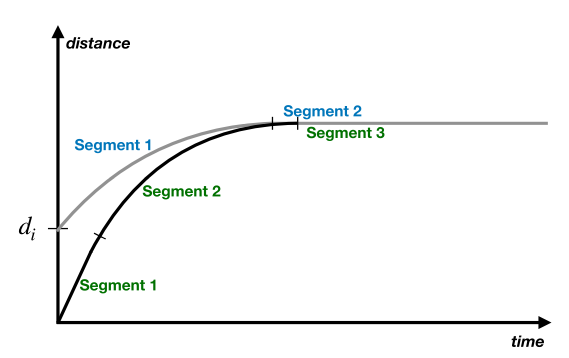
\includegraphics[width=8cm, height=4cm]{Figure-3.png}
    \caption{}
    \label{}
\end{figure}
\begin{block}{}
  There are potentially six ways of collision.All the five can be neglected when the distance in (2) is greater than distance in (5)
    \begin{align}
        d_{i} + \frac{v_{0}^2}{2 a_{i}} \leq v_{0} \tau + \frac{v_{0}^2}{2 a_{i+1}},\\
        \tau \geq \frac{d_{i}}{v_{0}} + \frac{v_{0}}{2}(\frac{1}{a_{i}} - \frac{1}{a_{i+1}}). 
    \end{align}
\end{block}
\end{frame}
\begin{frame}
\begin{block}{In case of $i \in I_{N}^{-}$\\}
 To provide a tight bound, the intersection of segment 1 of vehicle i and segment 2 of vehicle i+1 needs to be considered.
\end{block}
\begin{align}
    d_{i} + v_{0} t - \frac{a_{i} t^2}{2} = v_{0} t - \frac{a_{i+1} (t-\tau)^2}{2}
\end{align}
To guarantee that this touch actually happens between segments 1 and 2 of the trajectories, we need to make sure that the derivatives with respect to t at time $t_{c}$ of the expression at both sides are positive.\\
This happens when $t_{c} \leq \frac{v_{0}}{a_{i}}$\\
Using (8) we get 
\begin{align}
    \tau_{max}^{i,-} \leq \sqrt{\frac{2d_{i}(a_{i+1}-a_{i})}{a_{i+1}a_{i}}}
\end{align}
\end{frame}
\begin{frame}{Proposition-2}
  Safe breaking Probability Q justifies 
  \begin{align}
      Q^{*} = \prod_{i=1}^{N-1} [1-(1-p_{i})^{[\frac{\tau_{max}^{i}}{T}]}] \leq Q 
  \end{align}
  given that $\tau_{max}^{i} \geq T$ holds for each i\\
  \begin{block}{}
    Condition $\tau_{max}^{i} \geq T$ reflects the fact that at least one packet transmission attempt should be possible to get accomplished within a
feasible delay region.
  \end{block}
\end{frame}
\begin{frame}{Numerical Results}
  A V2V platooning protocol is currently being developed
within the European research project ENSEMBLE
\begin{figure}[h]
    \centering
    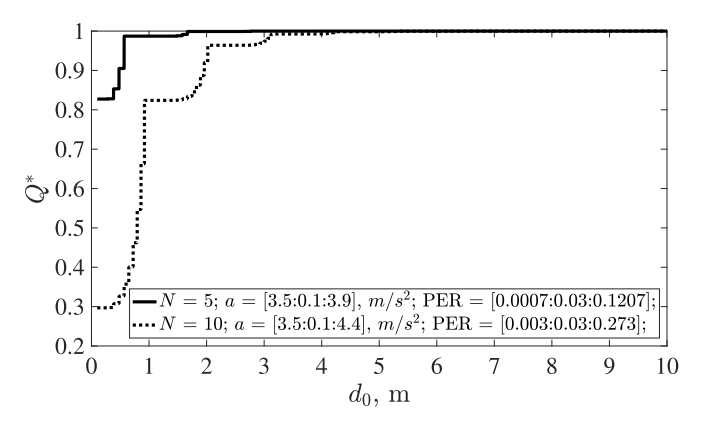
\includegraphics[width=10cm, height=6cm]{Figure-1.png}
    \caption{Platoon ordering(a_{1} < . . . < a_{i} < . . . < a_{N}) V_{0} = 22 m/s, f = 20 Hz}
    \label{}
\end{figure}
\end{frame}
\begin{frame}
\begin{block}{}
In above figure 
\begin{enumerate}
    \item vehicles are ordered according to their increasing
braking capability $a_{i}$.\\
\item results that even in shorter distance between the vehicles to reach Q close to 1.\\
\end{enumerate}
\end{block}
The communication scenario in a platoon exhibits in general
low PER due to that at least two antennas will be used on each
truck, mounted on each side of the cabin or in the wing mirrors.\\
$\implies$ more or less always line-of-sight between
transmitter and receiver antennas and the default output
power results in a favorable communication environment
\end{frame}
\begin{frame}
\begin{figure}[h]
    \centering
    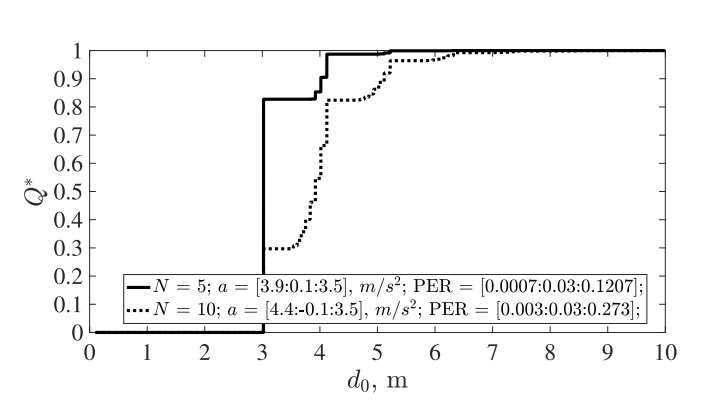
\includegraphics[width=10cm, height=6cm]{Figure-2.png}
    \caption{Platoon ordering(a_{1} > . . . > a_{i} > . . . > a_{N}) V_{0} = 22 m/s, f = 20 Hz}
    \label{}
\end{figure}. 
\end{frame}
\begin{frame}{}
Both Figures demonstrates the lower bound on the
safe braking probability, Q, for different inter-vehicular distances $d_{1} = \cdot
\cdot\cdot = d_{N} = d_{0}$
\begin{block}{}
In above figure
\begin{enumerate}
    \item the vehicles are ordered reversely in terms of
braking capability $a_{i}$\\
\item results in that longer distances are a necessity between the trucks to reach
a safe braking capability close to 1
\end{enumerate}
\end{block}   
\end{frame}
\begin{frame}
\begin{block}{Conclusion}
\begin{enumerate}
    \item Platooning holds great promise of increasing both road
traffic safety as well as efficiency but the functional safety
analysis of it is still benighted \\
    \item  The framework is used to evaluate the platooning protocol approach developed in the research project ENSEMBLE.Our numerical and analytical results reveal that the ENSEMBLE approach can reach a safe emergency
braking probability close to 1.
\end{enumerate}
  \end{block}
\end{frame}
\end{document}
